% !TEX root = ../../book.tex
\chapter{News Analytics: From Market Attention and Sentiment to Trading \label{chap:ch_news_an}}
\section{Introduction to News Analytics: Behavioral Finance and Investor Cognitive Biases}
 
 The determinants of large sporadic movements in stock prices that are not justified by fundamentals have been speculated and studied by many economists, starting with Keynes (1937)~\cite{keynes1937general}. The early empirical studies on this (see Cutler, Poterba and Summers (1989)~\cite{cutler1988moves}) linking stock news to stock prices did not find any significant relationships between the macroeconomic events and stock performance, particularly large returns. The rational financial theory that assumes that the market price of a stock is equal to the present value of future expected cash flows is generally unable to explain these patterns. So alternative explanations are sought from the behavioral finance perspective. It is argued that investors make decisions based on their sentiment that may not be related to data at hand about the stock performance. Generally, competing with these sentimental investors can be costly. Several market crashes can attest to these premises.
 
 
 There are a number of studies that find evidence to support the hypothesis that the content of news media can predict stock market activities. The communication channels have evolved from slow print media where the information is screened and edited to almost instantaneous social media, where participation is high but the information is of varying quality. The web which is in-between can be slower than social media but a certain degree of quality can be normally expected. Antweiler and Frank (2004)~\cite{antweiler2004all} find evidence for the relationship between internet message activities that can be characterized into ``buy'', ``sell'' or ``hold'' recommendations and the trading volume and the volatility.
 
 
 Tetlock (2007)~\cite{tetlock2007giving} provides an excellent summary of theoretical models of the effect of investor sentiment on stock prices. These models generally assume that there are two types of traders, noise and rational traders. Noise traders hold random beliefs about the future stock performance and rational traders hold informed beliefs based on the past performance of the stock and know the future potential. The difference between the two beliefs when measured right is taken to reflect the investor sentiment. The changes in the stock behavior can be due to a number of other factors as well, such as risk aversion, inventory management, etc. The so-called media pessimism can be a proxy for such stock-related or in general market-related factors as well but its timing is used to distinguish sentiment related influence on the stock behavior. Lower sentiment generally leads to downward pressure on prices resulting in low returns at short horizons but will be reversed in the long run. If it is due to true information about the stock, the trend in returns can be expected to persist. The investor sentiment is also likely to influence the trading volume with irrational traders trading heavily over ``rational'' traders with shorter horizon in mind. The empirical research clearly demonstrates the following: it is assumed that informed traders have access to information prior to it becoming widely known.
 	\begin{itemize}
	\item The firm's return on a news day positively predicts its returns after the news. The gradual dissipation of the liquidity shock after the news leads to return momentum.
	\item Returns on high-volume news days are better (positive) predictors of post-news returns than returns on low-volume news days.
	\item The contemporaneous correlation between the firm's trading volume and the magnitude of its price changes temporarily increases around news days.
	\item The price impact of informed trading in the firm's stock temporarily decreases as news reduces information asymmetry. 
	\end{itemize}
 
 
 Baker and Wurgler (2006)~\cite{baker2006investor} investigate how investors' beginning-of-period sentiment affects the cross-section of future stock returns. A number of proxies for sentiment are considered. These are closed-end fund discount measured by the difference between the net asset value of closed-end stock fund shares and their market prices, NYSE share turnover, the number and average returns of the IPOs, the equity share in the new issues and the dividend premium which is measured by the log difference of the average market-to-book ratios of payers and non-payers. These six proxies for investment are used to form a sentiment index via principal component method. The first principal component is then shown to be related to future stock returns after adjusting for the stock and firm characteristics such as firm size, age, profitability, book to market equity, etc.. The predictability of investor sentiment is stronger for high volatility, non-dividend paying, extreme growth and distressed stocks. Because the turnover measure is highly volatile, it is dropped from the index and the revised index values that are available are now based on the other five variables. Baker and Wurgler (2007)~\cite{baker2007investor} consider some additional proxies as well and these are able to better discriminate the two factors that could lead to mispricing, a change in sentiment of the irrational traders and a limit to arbitrage from the rational investors. Market turnover, defined as the ratio of trading volume to the number of listed shares, Market Volatility Index (VIX), equity issues as a ratio of total new issues that includes debt issues as well and a measure of insider trading pattern are all considered to be other proxies for the sentiment. The constructed index is orthogonalized to a set of state variables: real growth in durables, nondurables and services consumption; growth in employment and the National Bureau of Economic Research recession indicator. The time-varying index constructed from these is shown to match up well with the anecdotal accounts of the timing of bubbles and crashes.
 
 
It must be noted that the sentiment index constructed by Baker and Wurgler (2006, 2007)~\cite{baker2006investor}~\cite{baker2007investor} is based on monthly data as the underlying variables are somewhat slow-moving. At low frequency, the index does provide a predictive direction for the stock performance. The index is updated and posted in the authors' websites\footnote{\url{https://www.dropbox.com/s/ip2812eich83tw2/Investor_Sentiment_Data_20190327_POST.xlsx?dl=0}}; it is given in Figure~\ref{fig:sentimentindex}. Yu and Yuan (2011)~\cite{yuyuan} and Stambaugh, Yu and Yuan (2012)~\cite{stamb} show how the index can shed light on well-documented anomalies. These anomalies include unexpected deviations in performance during the time of financial distress; the firms with high probability of failure have lower, not higher, subsequent returns which is not expected by the standard asset pricing models. Another one is the momentum effect which refers to empirical observation that high past returns generally forecast high future returns. Also it is noted that higher past investment predicts abnormally lower future returns. 
	 \begin{figure}[!ht]
	\centering
	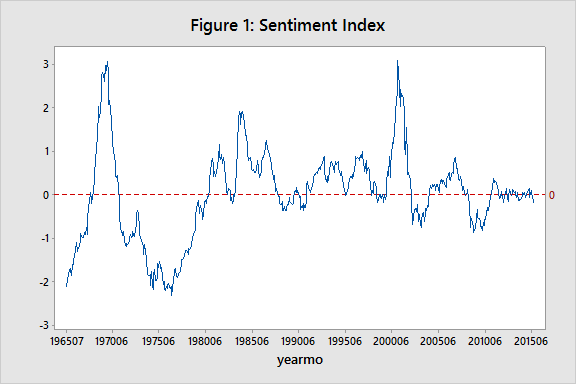
\includegraphics[width=\textwidth]{chapters/chapter_news_an/figures/ch4sec1sentimentindex.png}
	\caption{Sentiment Index.\label{fig:sentimentindex}}
	\end{figure}


While the extensive discussion of these results at the stock level is not possible here, we want to present the descriptive statistics of key performance indicators and other associated characteristics at the market level. The goal of this exercise is to show how conditional on the sentiment scores, the averages over different key characteristics differ. The data on Fama-French factor model, see Fama and French (2015)~\cite{fama2015international}, is taken from French's website.\footnote{\url{https://mba.tuck.dartmouth.edu/pages/faculty/ken.french/Data_Library/f-f_factors.html}} It consists of (details are directly from the site):


\begin{itemize}
\item SMB (Small Minus Big) is the average return on the nine small stock portfolios minus the average return on the nine big stock portfolios.

\item HML (High Minus Low) is the average return on the two value portfolios minus the average return on the growth portfolios.

\item RMW (Robust Minus Weak) is the average return on the two robust operating profitability portfolios minus the average return on the two weak operating profitability portfolios.

\item CMA (Conservative Minus Aggressive) is the average return on the two conservative investment portfolios minus the average return on the two aggressive investment portfolios.

\item $R_m - R_f$, the excess return on the market, value-weighted return of all CRSP firms incorporated in the US and listed on the NYSE, AMEX, or NASDAQ that have a CRSP share code of 10 or 11 at the beginning of $t$, and good return data for $t$ minus the one-month Treasury bill rate (from Ibbotson Associates).
\end{itemize}


The daily data on the above factors for the same duration as the duration of the sentiment data given in Figure~\ref{fig:varexcess} was collected and aggregated to match the monthly level sentiment data. For the excess return, $R_m-R_f$ we compute the monthly averages and as in Yu and Yuan (2011)~\cite{yuyuan}, we compute the realized variance of the excess return as,
	\begin{equation} \label{fig:varexcess}
	\widehat{\sigma}_t^2=\frac{22}{N_t}\sum_{t=1}^{N_t}(R_{mt}-R_{ft})^2,
	\end{equation}
where $N_t$ is the number of trading days in a month. The aggregated factors are plotted in Figure~\ref{fig:timefamafrench}.
 
 
	\begin{figure}[!ht]
	\centering
	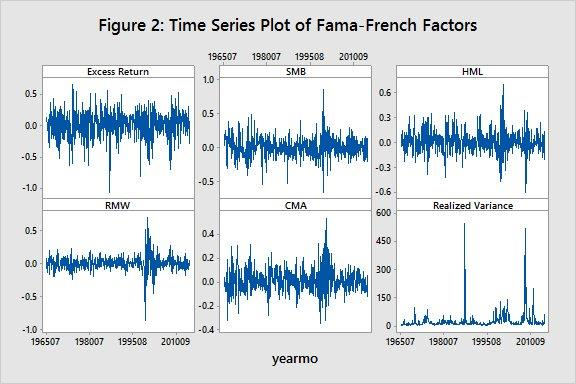
\includegraphics[width=\textwidth]{chapters/chapter_news_an/figures/ch4sec1famafrench.jpg}
	\caption{Time Series Plot of Fama-French Factors.\label{fig:timefamafrench}}
	\end{figure}


To classify the sentiment into low and high, Baker and Wurgler (2006)~\cite{baker2006investor} simply use the negative and positive scores. In order to allow for the natural variation in the sentiment scores, we classify the score below the first quartile ($-0.5$) as low sentiment and the score above the third quartile ($+0.5$) as high sentiment and in between as normal sentiment. Table~\ref{tab:famafrench} provides the summary of averages. The contrast between the low and high sentiment periods is quite evident.


        \begin{table}[!ht]
        \caption{Fama \& French Factors Across Sentiment Levels \label{tab:famafrench}}
        \begin{tabular}{lllll}
        & Low &     Normal      & High & All \\ \hline
        N & 152 &  283  & 168 & 603 \\
        Sentiment & -1.297 &  0.031  & 1.120 & 0.000 \\
        Excess Return & 0.0127 &  0.044  & -0.004 & 0.023 \\ 
        SMB & 0.031 &  0.009  & -0.010 & 0.009 \\
        HML & 0.014 & 0 & 0.052 & 0.018 \\
        RMW & -0.001 &  0.007  & 0.035& 0.013 \\
        CMA & 0.011 &  0.003  & 0.040 & 0.016 \\
        Realized Variance & 23.89 &  24.58  & 16.83 & 22.25
        \end{tabular}
        \end{table}


Some observations noted from the descriptive statistics follow: while the pattern in excess return is consistent with what is observed in Yu and Yuan (2011)~\cite{yuyuan}, the realized variance in high sentiment period is lower than the other periods, but this is consistent with the mean-variance relationship as expected by the asset pricing models. The SMB, which measures the difference in returns between small stocks and large stocks, is negative during high sentiment periods indicating the portfolio of small stocks does not do well in these periods. The HML, the difference in returns between high and low B/M stocks, tends to be positive and higher during high sentiment periods. The RMW, which measures the performance difference between robust and weak profitability portfolios, is also higher during high sentiment periods. Finally, CMA, which measures the difference in performance between conservative and aggressive firms, continues to do well in high sentiment periods.


Da, Engleberg, and Gao (2011)~\cite{da2011search} review studies on investor attention and its impact on stock performance. The proxies such as extreme returns, trading volume, news and headlines, advertising expense etc. were used as indirect measures of attention. Because some of these proxies can be driven by factors unrelated to investor attention, it must be noted that they, at best, are proxies. Instead it is suggested that search frequency of key words related to a stock in a search engine is a more direct measure of the attention as the users who search directly or indirectly express their intent and thus their interest.


Google publishes the search volume index (SVI) for the key words and except for rarely-searched tail terms, the index is fairly reliable due to the significant market share of Google in terms of search volume compared to volume from other search engines. Da et al. (2011)~\cite{da2011search} find SVI is a leading indicator of extreme returns and news and the abnormal SVI matches with the known anomalies. Generally, we must emphasize that what is meant by an anomaly. It is an empirical deviations from what is postulated by economic theory. A positive abnormal SVI generally predicts higher stock prices in the short term and price reversals in the long term. The SVI is correlated with other proxies of investors, particularly retail investors attention and it is available on a timely fashion. 


Da, Engleberg, and Gao (2015)~\cite{da2015sum} extend this idea to study the market-level sentiment and its correlation to aggregate market returns. The market-level index is based on the top thirty search terms that relate to general public's concern, such as unemployment, recession, bankruptcy, etc. The index is shown to predict short-term return reversals, increase in volatility and flows from equity funds to bond funds. The change in the index is demonstrated to be correlated with certain sentiment indicators, of Baker and Wurgler (2006)~\cite{baker2006investor}.


Stambaugh et al. (2012)~\cite{stamb} consider several asset-pricing anomalies that may be attributed to financial distress, momentum, asset growth etc. For each anomaly, the strategy that goes long in the highest-performing decile and goes short in the lowest-performing decile is examined. However as Huang et al. (2015)~\cite{huang} observe, ``\dots whether investor sentiment can predict the aggregate stock market at usual monthly frequency is still an open question.'' It must be noted that the market is efficient for the most part and any information gets impounded rather immediately at the higher frequency level. Thus there is a great deal of interest to mine news, attention and sentiment as they occur and the information from social media has come to play an an important role. We present some evidence to that effect in the next section. 



% Automated News Analysis and Market Sentiment
\section{Automated News Analysis and Market Sentiment}


As noted in Chapter~\ref{chap:ch_trading_fund}, trading now mostly occurs at a relatively high frequency level and hence any news related to a stock gets processed almost instantaneously. The literature reviewed in the last section refers to low frequency sentiment data and hence its influence on returns is not easy to notice. New technologies that can handle automatic news collection, extraction and categorization of relevant information are fast-emerging. Quantitative models that incorporate this information in investment decisions are being actively researched and automation of these activities can greatly help traders shorten their reaction time to emerging news feeds.


There has been a surge of academic interest in this topic (see Mitra and Mitra (2011)~\cite{mitra2} and Petersen (2016)~\cite{peterson}). Several technology companies (iSentium, SMA, MarketPsych, RavenPack, etc.) have sprung up in the last decade offering the service of aggregating the web information or sentiment, related to stocks. Financial news can be classified into two main groups. Some financial news related to a stock are released on a regular basis, such as earnings statements and models to analyze such events are well structured. The expectations on the earnings are formed based on the stock's other performance indicators and when the actual earnings differ from the trader's expectations, the trading decisions are normally adjusted for the a priori speculation. Then there are other news related to the product or personnel of the company that may come unscheduled and may affect the trading decisions. Although these are unstructured, they can also be easily processed. Usually the early exploiters of this type of information can expect to gain some advantage over others. These are generally termed as news-based event strategies and have been fairly well-studied in the finance literature. 


Unstructured news streams do not come at regular intervals and are qualitative and are usually in the form of a text. In order to correlate this information with the stock performance, they need to be appropriately quantified. Because this information originates from numerous sources such as in social media, it needs to be properly aggregated. Without any aggregation and smoothing, it may be difficult to extract the signal from the noise. Some common steps involved in making the news useable for trading are:
	\begin{enumerate}[--]
	\item Identify the unique, relevant and authentic news on a timely basis.
	\item Quantify the textual information into informative scores, whose variation would cover negative to positive sentiment/connotation.
	\item Aggregate the scores from different sources.
	\item Develop a baseline model adjusting for seasonality of the sentiment scores.
	\item Relate the abnormal deviation of the sentiment scores to abnormal stock price movements. 
	\end{enumerate}
As many of these concepts and related issues are discussed in the references cited in this chapter, we will be brief in our discussion. Das and Chen (2007)~\cite{daschen} show how it is possible to capture the net sentiment from positive and negative views on message boards using statistical natural language processing techniques. The emotive sentiment is elicited using different classification algorithms and the results are pooled via majority voting. Opinions are extracted from message board postings and they are classified into three types: bullish, bearish and neutral. The classification algorithms include parts of speech tagging and support vector machines. The algorithms are initially trained using humanly pre-classified messages and are designed to learn and apply these rules out-of-sample. Relating the sentiment to the performance of stocks in the Morgan-Stanley High-Tech Index it is observed that there is no strong relationship to individual stock prices but there is a statistical relation to the aggregate index performance. There is also a strong relationship between message volume and volatility consistent with Antweiler and Frank (2004)~\cite{antweiler2004all}. These examples clearly illustrate that investors sentiments expressed via media have some impact on stock behavior. 


We want to briefly provide some details on a few providers of web analytics; interested readers should consult these providers' websites for further details.

\begin{enumerate}[--]
\item Ravenpack (NewsScore): The key information on entities (company, organization, currency, commodities and place) from major news sources are gathered and processed for their relevance and are assigned event sentiment score. The scores are aggregated on a rolling window basis. In addition, the aggregate count as event volume, the event novelty score, event novelty elapsed time etc. are provided. For equity markets, composite sentiment score and the impact projections of the news are also available. The main news providers are Dow Jones Newswires, The Wall Street Journal (all editions) and Barron's. 

\item Thomson Reuters (News Analytics): Data fields include relevant score of the news item to the asset, number of sentiment words or tokens, sentiment classification, novelty of the content, feed volume etc. The sources are Reuters, PR Newswire etc. 

\item Thomson Reuters (MarketPsych Indices): News and social media information in real time are delivered as data series; there are categorized into three types of indicators: Emotional indicators, Macroeconomic metrics and Buzz metrics on the asset level. The data is updated on a minute basis. The social media data includes blogs, internet-forums and finance-specific tweets.

\item iSentium (iSense): Extracts sentiment signals using natural language processing architecture on Twitter data; the data feed includes retweets, if the author has a finance-related bio, number of followers etc. The impact is measured by the number of retweets for each author's tweets. 

\item Social Market Analytics (SMA): The data set provides a snapshot of sentiment factors at a 15~minute interval sources from Twitter/StockTwists messages. The raw scores are adjusted for the average and volatility. A measure of unusual volume activity is also provided. 
\end{enumerate}


In the next section, we will summarize studies that use the information provided by these agencies for developing trading strategies. To provide the theoretical underpinning of the effect of investor sentiment, two assumptions are made (see Delong, Shleifer, Summers and Waldmann (1990)~\cite{ssw}): market consists of two types of traders, noise and rational and they are both risk averse. Tetlock (2007)~\cite{tetlock2007giving} defines sentiment as the level of noise traders' random beliefs to rational traders' updated beliefs; it is argued that media (collective) pessimism is a proxy for either the sentiment or risk aversion. It is expected that high media pessimism will predict low returns at short horizons and at longer horizons, a reversion to fundamentals will occur. 



% News Analytics and its Applications to Trading
\section{News Analytics and its Applications to Trading}

We have reviewed select studies that have clearly documented the influence of news on stock market behavior. In this section, we will outline first the key methodologies used in relating the data on the inflow of news to key characteristics of stock trading and the stock performance indicators. A simple framework that we will follow is from Gloss-Klussmann and Hautsch (2011)~\cite{klub} and is depicted in Figure~\ref{fig:intervals}:
	
	\begin{figure}[!ht]
	\centering
	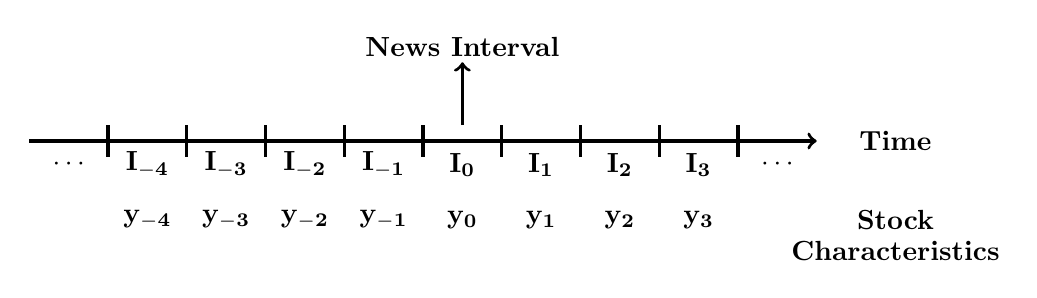
\begin{tikzpicture}
	\draw[very thick,->] (0,0) -- (10,0);
	\node at (11,0) {\textbf{Time}};
	\node at (0.5,-0.3) {$\cdots$};
	\node at (9.5,-0.3) {$\cdots$};
	\foreach \i in {1,...,9}
	{	
		\draw[very thick] (\i,-0.2) -- (\i,0.2);
		};
	\foreach \i in {-4,...,3}
	{
	
		\node at (\i+5.5,-0.3) {$\mathbf{I_{\i}}$};
		}
	\node at (11,-1) {\textbf{Stock}};
	\node at (11,-1.4) {\textbf{Characteristics}};
	\foreach \i in {-4,...,3}
	{
	
		\node at (\i+5.5,-1) {$\mathbf{y_{\i}}$};
		}
	\draw[very thick,->] (5.5,0.2) -- (5.5,1);
	\node at (5.5,1.2) {\textbf{News Interval}};
	\end{tikzpicture}
	\caption{News Intervals.\label{fig:intervals}}
	\end{figure}

The news arrival can generally be modeled as a point process but to remove any noisy friction in the data, both in the newsfront and in the stock price movement, it may be advisable to aggregate the information to short time intervals. The stock characteristics can include the return as well as volume, volatility, etc. during the interval. In addition to time aggregation, we also need to consider aggregation over different variables or dimensions of sentiment as in Baker and Wurgler (2006)~\cite{baker2006investor}. We describe these in two contexts below. \twomedskip


\noindent\textbf{Aggregation Over Dimensions:} \\


In the use of monthly data from Google, Da et al. (2015)~\cite{da2015sum} aggregate the daily change in a related search term, $i$, over the top thirty terms to come up with an index called, FEARS (financial and economic attitudes revealed by search) as 
	\begin{equation} \label{eqn:fears}
	\text{FEARS}_t = \sum_{i=1}^{30} R^i (\Delta \text{ASVI}_{it}),
	\end{equation}
where $\Delta \text{ASVI}_{it}$ is an adjusted (winsorized, deseasonalized, and standardized) daily change in search volume, 
	\begin{equation} \label{eq:asvi_it_ln}
	\Delta \text{ASVI}_{it} = \ln(\text{SVI}_{it}) - \ln(\text{SVI}_{it-1}).
	\end{equation}
Here, $R(\cdot)$ denotes the ranking function. Generally search volume data exhibits non-stationarity as well as strong weekday seasonality. It has, for instance, been found that web searches tend to be higher on Monday through Wednesday than on other days. The above adjustments to search volume take care of both concerns. Equation~\ref{eq:asvi_it_ln} is essentially a differencing operator that addresses the stationarity. A similar differencing for the weekday effect can be easily incorporated. These ideas were discussed in Section~\ref{sec:diffornot}.


The sentiment index in Baker and Wurgler (2006)~\cite{baker2006investor} is a composite index based on the five standardized sentiment proxies mentioned earlier. Because some variables take longer to express the same sentiment, the proxies are lagged. The series are smoothed over the prior twelve months and the index uses the $t-12$ value. As mentioned, the new series do not use turnover, due to fragmentation, NYSE is no longer the dominant venue. 


In the construction of this index, it appears the principal component of the five variables and their lags are used. Thus the first stage index has ten loadings; using the correlation between the index and current and lag values of the variables, the time index that is most appropriate for each of the variables is selected. In the original construction, the variables RIPO and PD-ND are lagged but the rest are used as of current time. The sentiment index is also further refined to adjust for a common business cycle components measured through growth in the industrial production index, growth in consumer durables, nondurables and services and an indicator variable for National Bureau of Economic Research (NBER) recessions. The resulting regression residuals, after adjusting for the time series effects, are argued as better, cleaner measures of sentiment. These are then used in the principal component analysis. Thus mathematically from Section~\ref{sec:s_dr}, if $x_t= (x_{1t}, x_{2t}, \ldots, x_{5t})'$, the first principal component $l'x$ is obtained by
	\begin{equation}
	\max_l \; l' \textstyle \Sigma_{xx} l \qquad \text{subject to} \quad l'l=1.
	\end{equation}
Because the variables here are standardized, it should be noted that the covariance matrix, $\Sigma_{xx}$ is also the correlation matrix. The first linear combination is associated with the eigenvector that corresponds to the largest eigenvalue of the matrix, $\Sigma_{xx}$, gives the sentiment score,
	\begin{equation} \label{eq:stsqlambda}
	s_t= \dfrac{l' x_t}{\sqrt{\lambda}}
	\end{equation}
in Figure~\ref{fig:intervals}. Here $\lambda$ is the largest eigenvalue of $\Sigma_{xx}$ so that the sentiment score, $s_t$ has unit variance. Because it is a standardized measure it is easy to interpret. \twomedskip


\noindent\textbf{Relating Sentiment to Stock Performance:} \twomedskip


The general framework relating the sentiment scores ($s_t$) to performance indicators ($y_t$) is simply through lagged regression. For example, the returns $r_t(y_t)$ are related to ($s_t$) and other control variables and can take the form:
	\begin{equation} \label{eq:rtkbetagamma}
	r_{t+k}= \beta_0 + \beta_1 s_t + \gamma' z_t + u_{t+k},
	\end{equation}
where $z_t$ is a set of control variables that may be related to the stock, such as Fama and French factors. The left side can also be (annualized) realized volatility, calculated by sampling the price over `$N$' times during a day. 
	\begin{equation}
	rv_t = 250 \sum_{d=1}^N r_{t,d}^2.
	\end{equation}
Because of the persistence of the volatility, some adjustments via differencing should be considered when relating sentiment scores to volatility. Finally, it is possible that the effect of positive sentiment on stock returns could be different from that of negative sentiment. Fitting models similar to \eqref{eq:rtkbetagamma} for both scenarios (positive and negative sentiment regimes) separately would be a worthwhile exercise. \twomedskip


\noindent\textbf{Aligned Investor Sentiment:} \twomedskip


In the above set-up, the construction of the sentiment scores (Equation~\ref{eq:stsqlambda}) or FEARS (Equation~\ref{eqn:fears}) is done first and then it is related to--for instance--the returns via \eqref{eq:rtkbetagamma} subsequently. Huang, Jiang, Tu and Zhou (2015)~\cite{huang} combine the two steps, together arguing the linear combination in \eqref{eq:stsqlambda} is constructed better in referencing to the stock characteristics and not on its own. They propose the partial least squares (PLS) method advanced by Wold (1984)~\cite{wold}. This method is similar to reduced-rank regression discussed in Section~\ref{sec:s_dr}. \twomedskip


\noindent\textbf{Partial Least Squares:} Partial least squares by Wold (1984)~\cite{wold} is an iterative computational algorithm for linear regression modeling, especially for situations where the number $n$ of predictor variables ($X_t$) is large. The $m \times 1$ multiple response, $X_t \;(m>1)$ version of partial least squares begins with a `canonical covariance' analysis, a sequential procedure to construct predictor variables as linear combinations of the original $n$-dimensional set of predictor variables $X_t$. At the first stage, the initial predictor variable $X_{1}^*=b_1'X_t$ is determined as the first `canonical covariance' variate of the $X_t$, the linear combination of $X_t$ that maximizes $\{(T - 1) \times \text{sample covariance of } b'X_t \text{ and } l'Y_t \} \equiv b' \mathbf{XY}' l$ over unit vectors $b$ (and over all associated unit vectors $l$). For given vectors $b$, we know that $l=\mathbf{YX'} b/(b' \mathbf{XY'YX'}b)^{1/2}$ is the maximizing choice of unit vector for $l$, so that we need then to maximize $b' \mathbf{XY'YX'}b$ with respect to unit vectors $b$. Thus, the first linear combination vector $b_1$ is the (normalized) eigenvector of $\mathbf{XY'YX'}$ corresponding to its largest eigenvalue. This follows easily from Result~\ref{res:6} in Chapter~\ref{ch:ch_mvts}. In the univariate case, $m=1$ and $\mathbf{Y}$ is $1 \times T$, and so this reduces to $b_1=\mathbf{XY'}/(\mathbf{YX'XY'})^{1/2}$ with associated ``eigenvalue'' equal to $\mathbf{YX'XY'}$.


At any subsequent stage $j$ of the procedure, there are $j$ predictor variables $x_{it}^*= b_i' X_t, i=1,\ldots, j$, are to be determined and the next predictor variable $x_{j+1}^*= b_{j+1}'X_t$; that is, the next unit vector $b_{j+1}$ is to be found. It is chosen as the vector $b$ to maximize the sample covariance of $b'X_t$ and $l' Y_t$ (with unit vector $l$ also chosen to maximize the quantity); that is, we maximize $b' \mathbf{XY'YX'}b$, subject to $b_{j+1}$ being a unit vector and $x_{j+1,t}^*=b_{j+1}; X_t$ being orthogonal to the previous set of $j$ predictor variables $x_{it}^*, i=1,\ldots,j$ (i.e. $b_{j+1}' \mathbf{XX'} b_i=0$, for $i=1,\ldots,j$). The number $r$ of predictors chosen until the sequential process is stopped can be taken as a regularization parameter of the procedure ; its value is determined through cross-validation methods in terms of prediction mean square error. The final estimated regression equations are constructed by ordinary LS calculation of the response vectors $Y_k$ on the first $r$ `canonical covariance' component predictor variables, $X_k^*= (x_{1k}^*,\ldots,x_{rk}^*)' \equiv \hat{B} X_k$, where $\hat{B}=[b_1,\ldots,b_r]'$; that is, the estimated regression equations are $\hat{Y}_k= \hat{A}X_k^* \equiv \hat{A}\hat{B} X_k$ with
	\[
	\hat{A}=\mathbf{YX}^{*'} (\mathbf{X}^* \mathbf{X}^{*'})^{-1} \equiv \mathbf{YX'} \hat{B}' (\hat{B} \mathbf{XX'} \hat{B}')^{-1}
	\]
and $\mathbf{X}^*=\hat{B}\mathbf{X}$ is $r \times T$. In practice, the predictor variables $X_k$ and response variables $Y_k$ will typically already be expressed in terms of deviations from sample mean vectors.


Discussion of the sequential computational algorithms for the construction of the `canonical covariance' components $x_{jk}^*=b_j'X_k$ required in the partial least squares regression procedure, and of various formulations and interpretations of the partial least squares method are given by Wold (1984)~\cite{wold}, Helland (1988,1990)~\cite{helland88}~\cite{helland90}, and Garthwaite (1994)~\cite{garth}. In particular, for univariate partial least squares, Garthwaite (1994)~\cite{garth} gives the interpretation of the linear combinations of predictor variables, $x_{jk}^*=b_j'X_k$, as weighted averages of predictors, where each individual predictor holds the residual information in an explanatory variable that is not contained in earlier linear combination components ($x_{ik}^*, i<j$), and the quantity to be predicted is the $1 \times T$ vector of residuals obtained from regressing $y_k$ on the earlier components. Also, for the univariate case, Helland (1988,1990)~\cite{helland88,helland90} showed that the linear combination vectors $\hat{B}=[b_1,\cdots,b_w]'$ are obtainable from nonsingular ($r \times r$) linear transformation of $[\mathbf{XY'},  (\mathbf{XX'})\mathbf{XY'}, \cdots, (\mathbf{XX'})^{r-1} \mathbf{XY'}]'$. One can notice the close similarity between reduced-rank regression and partial least squares. The former focuses on maximizing the correlation and the latter on maximizing the covariance.


Huang et al. (2015)~\cite{huang} demonstrate that the new combination of predictors based on PLS method has much greater predictive power for the aggregate stock market and its predictability is both statistically and economically significant. \twomedskip


\noindent \textbf{Social Media/Twitter Data:} Over the past years, significant development has been made in sentiment tracking technologies that can extract indicators of public mood from social media such as blogs and Twitter feeds. Although each Tweet is of limited number of characters, the aggregate of Tweets may provide an accurate representation of public sentiment. This has led to the development of real--time sentiment tracking tools (Opinion Finder, GPOMS (Google Profile of Mood Status), etc.) to track the public mood and relating them to economic indicators. Crowd--sourced data generated by social network sites such as Twitter/StockTwits is being increasingly used by quantitative researchers to generate trading signals. The wisdom of the crowd surprisingly appears to outperform the wisdom of the experts in a variety of instances. For a recent application relating sentiment data to earnings announcement, see Liew, Guo and Zhang (2017)~\cite{liewzhang}. We now illustrate a simple trading algorithm using the iSentium data.


iSentium expertise lies in providing market sentiment indicators. Market--related texts from Twitter are processed through Natural Language Processing Techniques and the contents are assigned sentiment scores in the range of $-30$ to $30$ with positive score indicating optimistic view and the negative score, a pessimistic view. For a specific keyword the data contains the following information: time when the Tweet is recorded, sentiment Score, total number of Tweets since Jan 1, 2012, whether it is a retweet, whether the author has a finance--related bio, number of followers of the author, number of Tweets posted by the author, and average number of retweets for each of the author's Tweets, measuring the author's impact.

In addition to per--tweet data, the company also provides binned data, binned over various time durations. Surprisingly tweet volume is high for popular ETFs and large cap technology stocks. To illustrate, we consider the per-tweet data from Jan 1, 2012 to September 10, 2014 for the \textbf{ESMini} (ticker symbol: \textbf{QQQ}). The typical data is listed in Table~\ref{tab:isentiumdata}:

        \begin{table}[!ht]
        \centering
        \caption{Typical Elements of iSentium Data \label{tab:isentiumdata}}
        \hspace*{-1.8cm}
        \begin{tabular}{rrrrrrrrrr}
        Date & Time & SS & Retw & Retwld & authid & FinBio & nfollow & ntweets & impact \\
        1/1/2012 & 3:04:41 & 9 & 0 & $-1.00\text{E}+00$ & 202647426 & 1 & 222 & 16 & 0 \\
        1/1/2012 & 3:10:06 & 9 & 0 & $-1.00\text{E}+00$ & 23059499 & 1 & 10501 & 27 & 0 \\
        1/1/2012 & 3:19:46 & $-11$ & 0 & $-1.00\text{E}+00$ & 202647426 & 1 & 222 & 25 & 0 \\
        1/1/2012 & 3:43:52 & 0 & 0 & $-1.00\text{E}+00$ & 202647426 & 1 & 222 & 30 & 0 \\
        1/1/2012 & 3:50:01 & 0 & 0 & $-1.00\text{E}+00$ & 23059499 & 1 & 10501 & 48 & 0 \\
        1/1/2012 & 4:10:01 & $-5$ & 0 & $-1.00\text{E}+00$ & 23059499 & 1 & 10500 & 89 & 0 \\
        1/1/2012 & 4:11:02 &  $-5$ & 0 & $-1.00\text{E}+00$ & 207429198 & 0 & 51 & 2 & 0 \\
        1/1/2012 & 4:12:10 &  $-5$ & 1 & $1.53\text{E}+17$ & 16704290 & 1& 1170 & 3 & 0 \\
        1/1/2012 & 4:26:07 & $-10$ & 0 & $-1.00\text{E}+00$ & 207429198 & 0 & 51 & 9 & 0 \\
        1/1/2012 & 4:30:03 & $-10$ & 0 & $-1.00\text{E}+00$ & 23059499 &	1 & 10500	 & 104 & $0.0625$ 
        \end{tabular}
        \end{table}


It is quite apparent from the short list of entries in Table~\ref{tab:isentiumdata}, the same author of a tweet can have varying sentiments in a short duration of time. It is also likely that a few authors can dominate the volume of tweets in a short duration ($\approx$90 minutes in the sample data in Table~\ref{tab:isentiumdata}). Consequently in the application we describe here, the daily summaries of sentiment scores are calculated and matched with the daily performance of ESMini. This, the sentiment data is smoothed so that extreme values are weighed in appropriately. Note that twitter activity occurs every day but the markets are open only on weekdays. No attempt is made to account for the cumulative effect of weekend sentiment scores on the beginning-of-the-week ESMini performance. The ESMini data contains daily price bars (with open, high, low and close) and the volume of transactions.


The time series plot of the sentiment related variables and the ESMini trade related variables are given in Figure~\ref{fig:sentimentesmini}. Here the variables are defined as:
        \begin{enumerate}[--]
        \item RetO$=\ln(P_{t \cdot 0}) - \ln(P_{t-1.0})$ based on opening price
        \item Volume is logged
        \item Volatility$= 0.5(H_t-L_t)^2 - 0.386(C_t-O_t)^2$, where $H_t=\ln(P_{t \cdot H})$, the high price observed during the day etc.
        \item SSAav is the average sentiment score for the day
        \item FBav is the proportion of tweets by the tweeters with a finance bio
        \item Retav is the average number of retweets per day 
        \end{enumerate}
While the focus is on sentiment score, the other two sentiment variables indicate the intensity of activity by the twitter participants in the finance field. 

	\begin{figure}[!ht]
	\centering
	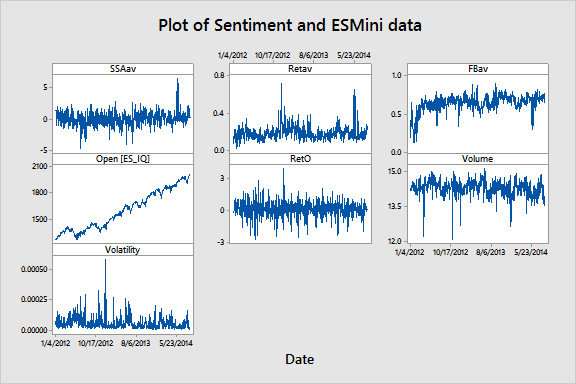
\includegraphics[width=\textwidth]{chapters/chapter_news_an/figures/ch4sec4sentimentesmini} 
	\caption{Sentiment score and ESMini. \label{fig:sentimentesmini}}
	\end{figure}


It can be seen from Figure~\ref{fig:sentimentesmini}, that the sentiment average (SSAav) exhibits some variation over time but it is generally stationary. There is some memory in the series as the first few autocorrelations are found to be significant. All the other sentiment related series also exhibit some memory. The same can be noted for the volume and volatility series as well. One of the key tools to connect two series in terms of lead-lag relationships is the cross-correlation function defined in Chapter~\ref{ch:ch_mvts} (see Section~\ref{sec:mutimserimod}). For the sentiment data ($s_t$) to be of any predictive use, it should be correlated to lead return ($r_{t+k}$) and lead volatility ($V_{t+k}$). Figures~\ref{fig:ccfssavreto} and \ref{fig:ccfssavvol} capture the cross-correlation, but one can observe that there is some concurrent correlation between $s_t$ and $V_t$. This may be due to the fact that the aggregation of data was done over the entire day, which may be too long a duration for aggregation of high frequency data. The traders may use any signals fairly quickly. These relationships can be confirmed in Table~\ref{tab:regesmini} with stepwise regression model fit. It can be observed all three variables: return, volume and volatility, are fairly well-explained by the sentiment data. 


	\begin{figure}[!ht]
	\centering
	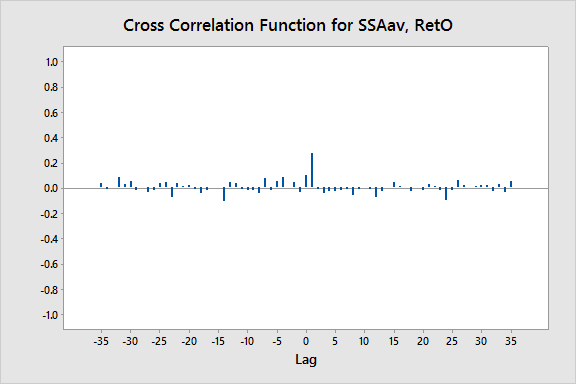
\includegraphics[width=\textwidth]{chapters/chapter_news_an/figures/ch4sec4crossfssaavreto} 
	\caption{CCF(SSAve $\rightarrow$ Reto). \label{fig:ccfssavreto}}
	\end{figure}

	\begin{figure}[!ht]
	\centering
	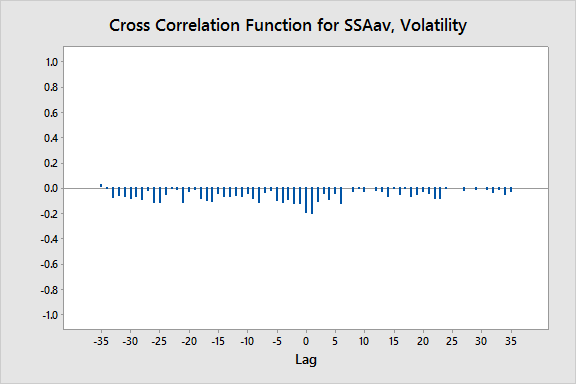
\includegraphics[width=\textwidth]{chapters/chapter_news_an/figures/ch4sec4ssaavvola} 
	\caption{CCF(SSAve $-$ Reto). \label{fig:ccfssavvol}}
	\end{figure}

	\begin{table}[!ht]
	\centering
	\caption{Regression of ESMini variables on sentiment factors \label{tab:regesmini}}
	\begin{tabular}{rrrr}
	\multicolumn{4}{c}{Response Variable} \\
	Predictors & Return & Volume & Volatility \\ \hline
	SSAav & --- & $-0.0482$ & $-0.00005$ \\
	SSAverlag & $0.1895$ & $-0.0291$ & $-0.00006$ \\
	AuHTAV & --- & $-0.000017$ & $-0.000001$ \\
	RetAV & --- & --- & $-0.000063$ \\
	NfollowAV & --- & --- & $-0.000001$ \\
	AVetW & --- & --- & $0.000047$ \\
	Constant & $0.0759$ & $14.41$ & $0.000085$ \\ \hline
	$R^2$ & $0.0732$ & $0.1154$ & $0.1357$ \\ \hline
	\multicolumn{4}{c}{$\ast$All indicated factors are significant at 0.05 level}
	\end{tabular} 
	\end{table}

Two na\"ive strategies can be proposed for trading using the sentiment data; both are in the spirit of the discussion related to sentiment data by Baker and Wurgler (2006)~\cite{baker2006investor}. The first strategy develops rules based on the sentiment scores and the second is based on the more direct regression relationship between returns and the sentiment scores: 

\begin{enumerate}[1.]
\item Crossover Strategy: If the difference between 3-day EWMA and 30-day EWMA of sentiment scores is positive, go long; otherwise go short. 
\item Open-to-open Strategy: Regress open-to-open returns on 10-day EWMA and its lag to predict the return; if positive, go long, hold the position until the next day open. 
\end{enumerate}


It is easy to note that the crossover strategy is similar to the moving average oscillator rule, discussed in Chapter~\ref{ch:stat_ts}, comparing the short term trend with the long term trend. The strategy exploits the deviation between the two. Both strategies can be evaluated on a moving window basis. Here we present results for the cross-over strategy only. As noted from Figure~\ref{fig:sentimentesmini}, the ESMini price has been steadily going up and thus a simple buy and hold strategy over time would be profitable. So we compare performance of the strategy with the buy and hold. The simple averages over buy and sell signals are quite revealing as seen from Table~\ref{tab:descstatcross}

        \begin{table}[!ht]
        \centering
        \caption{Descriptive Statistics (Averages): Cross-over strategy \label{tab:descstatcross}}
        \begin{tabular}{rrrrrrrr}
         & SSAve & RetAve & FBAC & Reto & Volume & Volatility & $N$ \\
        Short  & $-0.5223$ & $0.1783$ & $0.6539$ & $-0.0866$ & $14.327$ & $0.000061$ & 333 \\
         Long & $0.4398$ & $0.1793$ & $0.6477$ & $0.2206$ & $14.220$ & $0.00044$ & 309 \\
         All & $-0.0592$ & $0.1788$ & $0.6509$ & $0.06125$ & $14.28$ & $0.000053$ & 642
        \end{tabular} 
        \end{table}

The negative signal from sentiment score matches with the negative return and higher volatility. The averages are in the right direction. The equity curve in Figure~\ref{fig:equitycross} clearly demonstrates the value of this strategy. \twomedskip

        \begin{figure}[!ht]
        \centering
        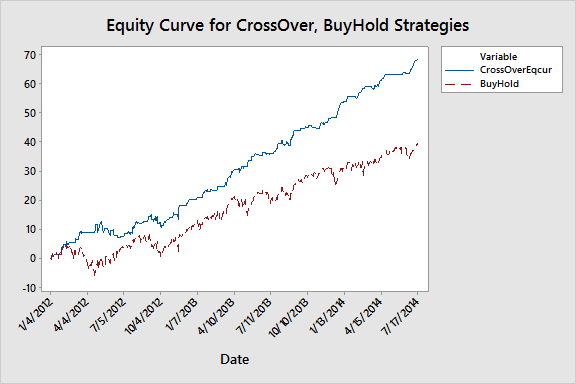
\includegraphics[width=\textwidth]{chapters/chapter_news_an/figures/ch4sec4equitycross} 
        \caption{Equity Curve for ESMini. \label{fig:equitycross}}
        \end{figure}

\noindent \textbf{Bloomberg News and Social Sentiment Data:} The news agency applies statistical machine-learning techniques to process the textual information related to equities and quantifies the sentiment both at the (news) story-level and at the equity-level. The scores indicate at the story-level if the sentiment is positive, negative, or neutral with a confidence level; these are aggregated to provide the company-level sentiment. The computation is based on both news and Twitter feeds with a rolling window of half-an-hour. The predictive strength is tested out using the performance of the equity at a daily level as well as through changes in the stock price during the day. The approach is similar to cross-sectional momentum strategy that is outlined in Chapter~\ref{ch:stat_ts}. It can be shown that the stocks in the top decile of the day's sentiment scores tend to do better during that day. 


The sentiment data also can be used to predict the nature of earnings report. The event driven strategies are still a significant part of trading strategies and it can be shown that sentiment scores prior to earnings releases can augment these strategies. The intraday strategy is based on using the arrival of information during an interval of pre-defined duration and making trading decisions based on the sentiment scores and their confidence. Generally traditional news combining with a twitter feed can generate stronger signals. A methodology used to relate sentiment scores whether from traditional news or from twitter is to first construct an index, 
	\begin{equation}\label{eqn:itwithln}
	I_t= \ln\left( \dfrac{1+\| BV_t \|}{1+\| BE_t \|}\right)
	\end{equation}  
that adjusts for the baseline activities, here $BV_t$ denotes the number of bullish tweets and $BE_t$ denotes the number of bearish tweets. Defining the intraday return, $r_t= \ln(P_t^{\text{close}}) - \ln(P_t^{\text{open}})$, where $P_t$ refers to the stock price on a given time unit. Then forming, $y_t=(I_t^N,I_t^{TW},r_t)'$, VAR model that was discussed in Chapter~\ref{ch:ch_mvts} is used to identify the lead-lag relationships; here $I_t^N$ is the index for the news sentiment, such as Google search volume for relevant keywords and $I_t^{TW}$ refers to the index based on Twitter data. The VAR model provides a broader framework to consider other information such as market volume, market volatility, etc. that can be easily incorporated. \twomedskip


\noindent\textbf{Thomson Reuters MarkerPsych Indices (TRMI):} The TRMI are also based on news and social media that produce three key types of indicators: Emotional indicators, Macroeconomic metrics and the so-called Buzz metrics. These are updated on a minute basis and covers various economic entities. The indices cover over fifty items and they are scored from $-1$ to 1 or from 0 to 1. Due to space constraints, we are not able to cover each source in depth. The comparative value of different sources of sentiment data could be of interest.


We want to conclude this section by noting some recent research that further demonstrates the use of sentiment data in trading. First Constantinos, Donkas and Subrahmanyam (2013)~\cite{contdonksub13} establish a link between sentiment and momentum. The news diffuses through the actions of various `newswatchers' and creates momentum, which was previously attributed to mainly past price movements. Reactive trading gets corrected when momentum positions are reversed as the difference between fundamental information and the news becomes apparent. It is argued that those who follow news closely will under-react if the information contradicts their sentiment. This means that bad news among loser stocks will diffuse slowly where sentiment is optimistic. The sentiment measure that is used is the widely recognized conference Board's Consumer Confidence index. The central hypothesis that sentiment impacts momentum via cognitive dissonance is generally supported by the empirical analysis.


The statistical arbitrage rules developed in Chapter~\ref{ch:stat_ts} are widely used in industry. They exploit market anomalies whether they are due to fundamental news or sentiments. The sentiments can lead to mispricing of assets. The efficacy of technical analysis and how it is related to investor sentiment is also studied in Smith, Wang, Wang and Zychowicz (2016)~\cite{smithwangwangzy16} by focusing on its usage by the sophisticated group of traders, the hedge fund managers. 


It is observed that one in five hedge funds employ technical analysis. The hedge fund managers integrate both fundamental and technical analysis in their decision-making process on market timing. Sentiment analysis is shown to be an important catalyst in this regard. It is documented that the performance of technical analysis users is better than nonusers in high-sentiment periods but technical tools are less valuable during low sentiment periods. The sentiment data is found to be very useful for market timing. The idea of using sentiment data for return movements has been extended to other dimensions as well. \\


\noindent\textbf{Manager Sentiment Index:} It should be expected that the corporate manager's sentiment could play a role in the investment decisions as they may have informational advantage over outside investors. As they are humans, some behavioral biases are likely to be present. Investors may simply follow managers reading of financial disclosures. Jiang, Lee, Martin and Zhou (2019)~\cite{jianleemartin} construct a manager sentiment index from the textual tone in conference calls and in financial statements related to the firm as it reflects manager's subjective views. The measure is the difference between the positive and negative words standardized by the total word count on a monthly basis. This new index is shown to predict future aggregate stock returns consistent with theory and its predictive power is shown to be greater than other macroeconomic predictors discussed earlier. The proposed index can act as complementary to other investor sentiment measures. 



% Discussion / Future of Social Media and News in Algorithmic Trading
\section{Discussion / Future of Social Media and News in Algorithmic Trading}

We have presented in this chapter summaries of studies that clearly document the efficacy of the statistical arbitrage in high-sentiment periods when the short-sale constraints can discourage the elimination of overpricing that may be due to sentiment. The benefits seem to disappear in the low-sentiment periods. These results are quite robust and stand true in different volatility regimes as well. The momentum rule results in profits when investors are optimistic which happens during high sentiment periods. Large investors can read this better and promptly sell likely losing stocks in optimistic periods.


In a recent article, Zhou~(2018)~\cite{zhou18measure} discusses open issues related to measuring and using investor sentiment. First is related to aggregating various proxies of available sentiment measures. The aggregation by PCA captures only the total variance in the proxies but does not necessarily relate to the investment characteristics. An alternative is to use PLS or canonical correlation methods to find the optimal aggregation of the sentiment measures but this can change over time. The problem is somewhat related to combinations of forecasts, discussed in Section~\ref{sec:multindboostmeth}. In the use of iSentium data, we dealt with the time aggregation of individual sentiment scores with simply averaging them. Each tweet contains other information such as retweets, number of followers and whether the tweeter has a finance bio, etc.. All these additional details may capture the reliability of a sentiment score and so deserve further attention. 


The second issue mentioned is to carefully study the relationship between technical rules-based sentiment (which results in momentum or contrarian strategies) and other sentiment measures. One indicator that is based on technical analysis is
	\begin{equation}\label{eqn:williams}
	\text{Williams \% }R= \dfrac{\text{highest high}-\text{closing price}}{\text{highest high}-\text{lowest price}} \times 100.
	\end{equation}
The above is calculated based on the past ten days and indicates if a stock is overbought or oversold, which may be the result of executive optimism or pessimism. If the above measure is less than 20, it is taken to indicate that it is `overbought' and if it is greater than 80, it is taken as `oversold'. The idea is similar to the oscillator index discussed in Chapter~\ref{ch:stat_ts}. 


Finally, which sentiment features are useful to forecast asset returns? What does the volatility in sentiment mean? How long does the memory in sentiment last? These are open issues that need further investigation. There is a growing concern about the quality of news or information as we move from print media to web to social media. News, good or bad, travels faster now; the news distribution platforms have reduced market entry costs and the goal is to simply maximize traffic. This also results in weakening of knowledge editors as quality control intermediaries. Non-regulatory initiatives such as fact-checking and codes of conduct do seem to correct for potential failures. Online consumption of news is now channeled through platforms such as search engines, news aggregators and social media. These are mostly algorithm-driven. Although editors retain control over the content, they do not control the reach to potential readers. A recent estimate of print media shows only 32\% get their news through print and the rest gather their news through web related media. Search engines are subject to manipulation. Now users are spending more time to interact with each other via social media. Content can propagate via stronger network links between users. But the content editors role seems to be greatly diminished. While these observations are made in the context of general information, in-depth studies in the context of financial markets are called for. But the influence of news media on the stock market behavior remains to stay.